% !TeX spellcheck = en_US
% !TeX encoding = UTF-8
\chapter{Data Collection-Subject Study}

A collaborative assembly task involving wooden pieces was designed in the robot laboratory of the Institute of Control Theory and Systems Engineering at the Technical University of Dortmund. This setup aimed to accurately replicate the types of tasks commonly seen in industrial settings where collaboration between humans and cobots is frequently observed. The Universal Robot UR10 was selected as the cobot to be used in the study. A call for participants invite was sent out, and 20 male students who all had a technical background volunteered to participate in the study. 17 of the students did not have any previous experience working with a robot in any way, whereas the remaining
had some previous experience with robots. All of them were between the ages of 21-28. Before the experiment began, all participants were given a comprehensive overview of the study's objectives and procedures, along with a consent form. Only those participants who agreed to the terms and signed the consent form were permitted to proceed with the experiment. To ensure the ethical integrity of the study, a prior request for ethical approval was submitted to the appropriate ethics council (to be added) and permission was obtained to conduct the subject study.

\section{Design of Tasks}
Since we wanted to replicate an industrial assembly task, assembly of various mock items using wooden children's toys was selected. The effect of stress on different factors was to be investigated. These include three distinct levels of robot collision avoidance strategies:

These included three distinct levels of different collaboration levels:

\begin{itemize}
    \item \textbf{Different Workspace}:
    Human and cobot have no overlapping space. The robot works in the background.
    
    \item \textbf{Shared Workspace}:
    Where the Human and cobot share the same work area, and the robot brings the item for the assembly tasks to the human and places it in the work area.
    
    \item \textbf{Shared Workspace with Direct Collaboration}:
    Where they share the same area, and the robot brings the item, and there is a direct handover of the items to the human.
\end{itemize}

As well as three robot collision avoidance strategies:

\begin{itemize}
    \item \textbf{No Collision Avoidance}:
    No collision avoidance measures are in place, and the robot stops at a collision.
    
    \item \textbf{Dynamic Collision Avoidance}:
    The robot identifies the human as a dynamic obstacle and adjusts its trajectory to avoid collisions.
    
    \item \textbf{Predictive Collision Avoidance}:
    This strategy uses predictions to predict the human's future position and adjusts its trajectory to avoid collisions.
\end{itemize}

The table \ref{table:tasks} shows the various combinations of factors and their naming conventions, yielding a total of seven experimental scenarios since collision avoidance is not applicable when different workspaces are involved. So a within-subject design was employed where each participant was tested on all seven scenarios.By having the same participants perform each task, we minimized the impact of differing skill sets, experiences, and cognitive abilities, which could otherwise skew the results.

\begin{table}[h]
    \centering
    \renewcommand{\arraystretch}{2}
    %\resizebox{\columnwidth}{!}{%
    \begin{tabular}{|c|c|c|c|}
    \hline
    \textbf{\makecell{Collision Avoidance \\ Strategy}} & \textbf{\makecell{Different \\Workspace (A)}} & \textbf{\makecell{Shared \\Workspace (B)}} & \textbf{\makecell{Shared Workspace with \\ Direct Collaboration (C)}} \\ \hline
    \textbf{\makecell{No Collision \\Avoidance (X)}} & AX  & BX  & CX \\ \hline
    \textbf{\makecell{Dynamic Collision \\Avoidance (Y)}}        & Not Available                               & BY                           & CY                                                    \\ \hline
    \textbf{\makecell{Predictive Collision \\Avoidance (Z)}}    & Not Available     & BZ                           & CZ                                                    \\ \hline
    \end{tabular}
    
\caption{Task names for different Collision Avoidance Strategies and Workspace Scenarios}
\label{table:tasks}
\end{table}


To avoid any potential learning effects and ensure that each task measures the intended variables accurately, we had to design 7 different assembly tasks. Each task involved assembling a unique item, carefully chosen of similar complexity and required effort. This similarity in task difficulty was crucial to avoid the introduction of other variables which could skew the results. Figure \ref{fig:task} shows the final assemblies completed in each of the seven tasks.By standardizing the complexity across tasks, we aimed to isolate the impact of the collision avoidance strategies and collaboration levels. We also had to consider potential order effects, we counterbalanced the sequence of tasks, ensuring that learning or fatigue did not affect the outcomes in any way. Each participant experienced the tasks in a unique order, balancing out any potential biases introduced by the order of task presentation. 

\begin{figure}[h]
	\centering
	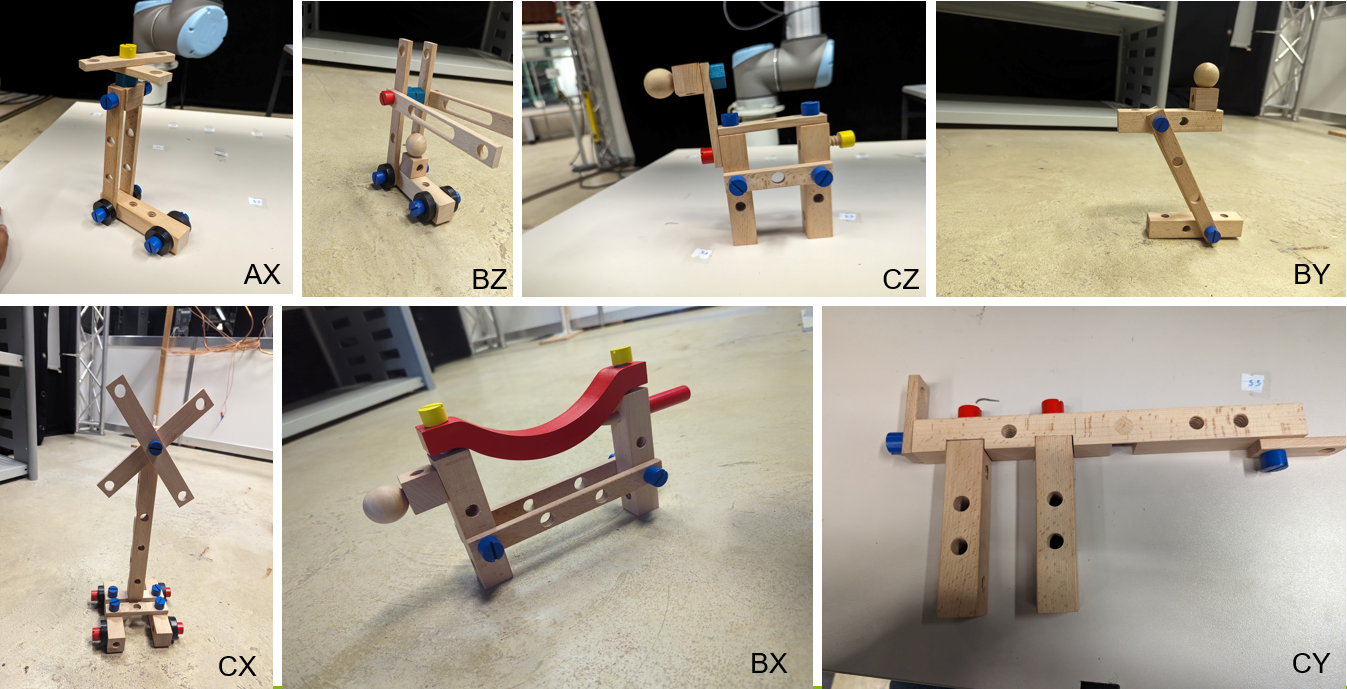
\includegraphics[width=\columnwidth]{images/7tasks.png}
	\caption{7 different assembly tasks}
	\label{fig:task}
\end{figure}

\section{Apparatus and Experimental Setup} 
The experiment was set up in a specially designated area of our laboratory. At the center of this arrangement was the collaborative workspace, featuring a table and chairs for the human participant (Area B in Fig \ref{fig:setup}), positioned directly opposite the robot's dedicated area. Adjacent to this, on the right side of the collaborative workspace, a table was placed to hold the various items needed for the assembly tasks(Area A Fig\ref{fig:setup}). The robot would pick the necessary items from this table for each specific task and deliver them to the human participant. In front of the human participant, a mobile device was also placed. This device was key to the experiment, as it presented the participant with concise, step-by-step instructions for each assembly task. These instructions were visually displayed, offering clear and easy-to-follow guidance. 

Figure \ref{fig:setup} shows the experimental setup. 

 

\begin{figure}[h] 

    \centering 

    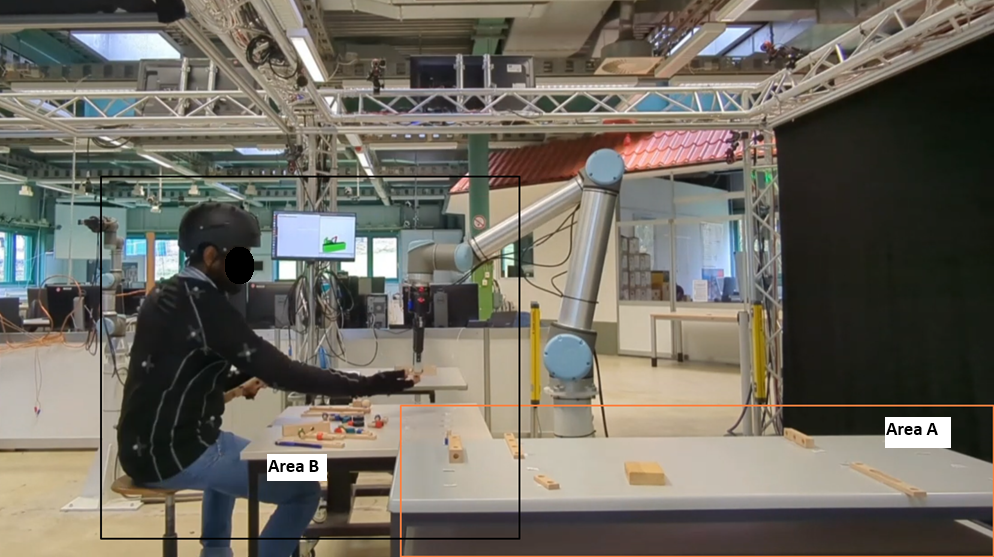
\includegraphics[width=0.9\columnwidth]{images/Setup.png} 

    \caption{The experimental setup} 

    \label{fig:setup} 

\end{figure} 



The entire experimental area had an advanced OptiTrack motion capture system, outfitted with 12 high-precision cameras. These OptiTrack cameras, known for their exceptional accuracy and low latency are used to capture every detail of the human participant's movements. This setup was necessary in providing a detailed and continuous record of the participant's interactions with the robotic system, also aiding the collision avoidance trajectory planning for the robot. The use of the OptiTrack system enabled us to gather precise data on human motion and behavior, crucial for analyzing the efficacy and safety of human-robot interaction in assembly tasks. The participants were equipped with the motion capture suit which had 25 distinct marker points which were used to capture the human's head and upperbody. For safety purposed the participant had also been given a helmet to wear.
For capturing the physiological signal of the participants, the Empatica E4 wristband was equipped in the participants non-dominant hand.


\begin{figure}[h]
	\centering
	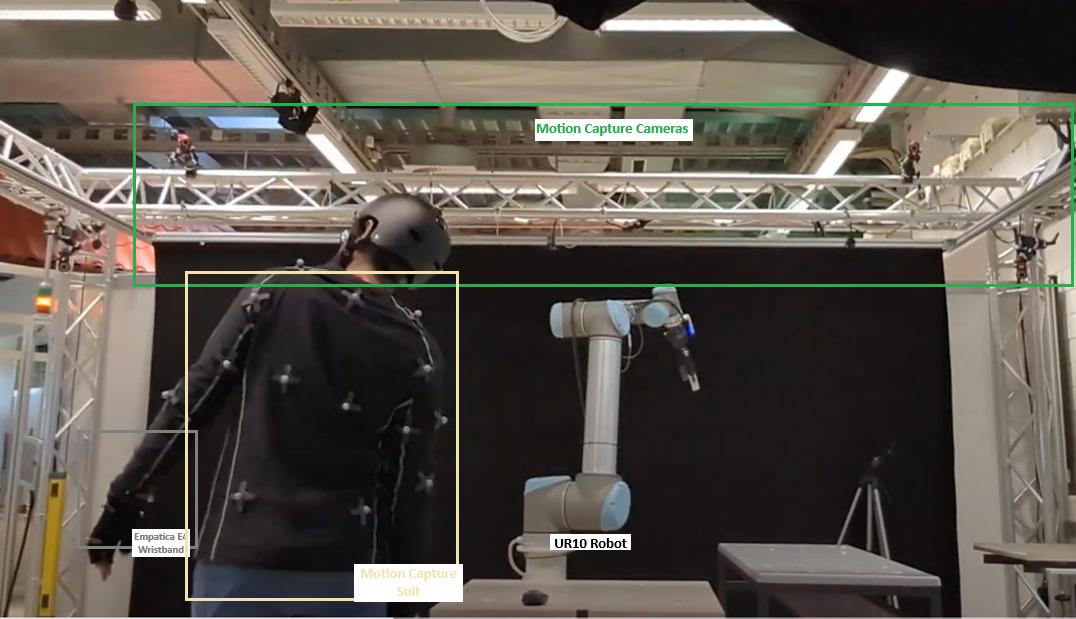
\includegraphics[width=0.9\columnwidth]{images/apparatus.png}
	\caption{Apparatus used}
	\label{fig:apparatus}
\end{figure}


\section{Procedure/Protocol}
(With the diagram in the ppt)
Experimental procedure At the beginning, each group of participants was briefed about the objectives and the detailed procedure of the experimental study. Secondly, participants were conducted to their work-area where they were given detailed information of the assembly process to perform. Meanwhile, the participant in charge of assembly was equipped with the Empatica E4 on the left wrist and a 15 min wait period was observed to ensure an appropriate adherence of the electrodes, so as to acquire reliable EDA data. Next, the participant was asked to relax and stand still to record 2 min of “baseline”, i.e., the physiological signals at rest. Next, the repetitive assembly process was randomly selected in one of the two modalities (i.e., Manual or HRC) and began for a 4 h work-shift. A 10 min break was also scheduled after 2 h of work, in order to simulate real-life working conditions. The other two participants monitored the whole process by recording process failures and product defects. At the end of the 4 h work-shift, general unstructured feedbacks on the experiment were collected. In the second shift, the same procedure was followed for the remaining modality (i.e., HRC or Manual). Therefore, each group of participants performed